%//==============================--@--==============================//%
\subsection{Energia e Potência. Diagrama de carga}
\label{subsec:energy-and-power}

A relação básica entre energia e potência exprime-se por:
$$
    P = \frac{dW}{dt} \qquad\rightleftarrows\qquad W = \int P\, dt
$$
onde $W$ denota a energia (expressa em joule, J) e $P$ a potência (expressa em watt, W).

\vspace{1em}
\noindent A carga de um Sistema de Energia Elétrica (SEE), varia significativamente ao longo do dia, acompanhando a atividade humana. Para um diagrama de carga define-se
$$
    h_d = \frac{W}{P_\text{max}}\, [\text{unidades de tempo}] \qquad\quad\qquad f_d = \frac{P_\text{med}}{P_\text{max}}\, [\%], \mkern9mu \text{em que } P_\text{med} = \frac{1}{T} \int_T P\, dt
$$
a \textit{utilização diária da ponta}, $h_d$, como a relação entre a energia e a potência máxima; e também o \textit{fator de carga diário}, $f_d$, como relação entre a potência média e a potência máxima.

\begin{figure}[H]
    \centering
    \scalebox{0.9}{%
        \begin{tikzpicture}
            \begin{axis}[
                xlabel={Horas}, xmin=0, xmax=24,
                xtick={0,2,4,6,8,10,12,14,16,18,20,22,24},
                ylabel={Carga $[$MW$]$}, ymin=0, ymax=50,
                ytick={0,5,10,15,20,25,30,35,40,45,50},
                grid=both,
                minor tick num=1,
                width=10cm,
                height=6.5cm
            ]
            
            \addplot [thick, line width=1.5pt, fill=gray!20, fill opacity=0.45] table [col sep=comma, x=Time, y=Load] {src/1/data.csv} \closedcycle;

            \addplot [mark=*, mark size=2pt, only marks] coordinates {(13, 41)};
            
            \node[above right, fill=white, fill opacity=0.6, text opacity=1, font=\large] at (13,41) {$P_\text{max}$};

            \node[above right, font=\large] at (10,10) {$W = \displaystyle \int P\, dt$};

            \draw [dashed, line width=1.25pt] (axis cs:0, 30.12) -- (axis cs:24, 30.12);

            \node[above, fill=white, fill opacity=0.6, text opacity=1, font=\large] at (4,30) {$P_\text{med}$};
            \end{axis}
        \end{tikzpicture}
    }
    \caption{Exemplo de diagrama de carga (diário)}
    \label{fig:diagrama-carga}
\end{figure}
%//==============================--@--==============================//%
\subsection{Potência em Sistemas de Energia Elétrica}
\label{subsec:power-SEE}

Os SEE atualmente funcionam quase na sua totalidade em corrente alternada --- com uma frequência de $50$ Hz na Europa e de $60$ Hz nos EUA e no Brasil ---, existindo casos especiais em que se utiliza a corrente contínua.\cite{paiva2005}

\renewcommand{\thefootnote}{\fnsymbol{footnote}}
\footnotetext[4]{%
    Em alguns países, como por exemplo no Japão, coexistem as duas frequências.
}
\renewcommand{\thefootnote}{\arabic{footnote}}

%//==============================--@--==============================//%
\subsubsection{Potência Instantânea, Potência Ativa e Reativa, Potência Complexa e Aparente}

Considerando um sistema monofásico constituído por um gerador que dá origem a uma tensão $v$ aos terminais de uma carga representada por uma impedância constante $Z$, define-se a \textit{potência instantânea} transferida do gerador para a carga como
$$
    \begin{aligned}
        p = v i &= \overbrace{\sqrt{2}V \cos(\omega t + \alpha_v)}^{\text{tensão }v} \cdot \overbrace{\sqrt{2}I \cos(\omega t + \alpha_i)}^{\text{corrente }i}, \qquad \forall (\alpha_v, \alpha_i) \in [0,2\pi] \times [0,2\pi]: \phi \in [-\pi/2,\pi/2] \\
        &= VI \cos(\phi) - VI \cos(2\omega t - \phi)
    \end{aligned}
$$
em que $\phi = \alpha_v - \alpha_i$ (desfasagem da tensão face à corrente). Massajando a expressão conclui-se
$$
    p = \underbrace{VI \cos(\phi) [1 - \cos(2 \omega t)]}_{p_1} - \underbrace{VI \sin(\phi) \sin(2\omega t)}_{p_2}
$$
Repare-se que a componente $p_1$ tem valor médio constante e $p_2$ tem valor médio nulo. A \textit{potência ativa} é o valor médio da potência instantânea, e corresponde portanto à potência efetivamente transferida:
$$
    P = VI \cos(\phi) \quad [\text{W}]
$$
A \textit{potência reativa} é o valor máximo da componente da potência que oscila entre o gerador e a carga, cujo valor médio é nulo, resultante da variação da energia magnética/elétrica armazenada nos elementos da carga:
$$
    Q = VI \sin(\phi) \quad [\text{VAr}]
$$
\noindent \textbf{Nota}: A grandeza $\cos(\phi)$ designa-se por \textit{fator de potência}, $fp \delequal P/S = \cos(\phi)$.

\clearpage
\vspace*{-2.25em}
\begin{centering}
    \begin{minipage}[b]{0.5\linewidth}
        \begin{figure}[H]
            \centering
            \scalebox{0.925}{%
            \begin{circuitikz}[scale=1.25]
                % Voltage source
                \draw (0,0) to[sV] (0,2.75) -- (4,2.75);
                % Arbitrary impedance (Z)
                \draw (4,2.75) node[circ] {} to[generic, l=$Z$, v=$v$] (4,0) node[circ] {}  -- (0,0);
                % Draw the current's arrow
                \draw[-latex, black, line width=0.9pt] (1.25,2.9) -- (2.75,2.9) node[midway,above] {$i$};
                % Label
                \draw (-0.35,0.7) node[xshift=0mm, yshift=2mm] {$(\omega)$};
            \end{circuitikz}}
            \caption{Sistema monofásico em corrente alternada}
        \end{figure}
    \end{minipage}%
    \begin{minipage}[b]{0.5\linewidth}
        \begin{figure}[H]
            \centering
            \scalebox{0.925}{%
            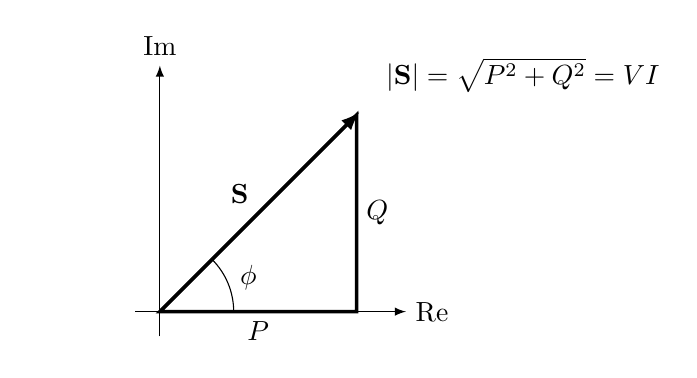
\begin{tikzpicture}[scale=1.25, >=latex]
                % Draw real and imaginary axes
                \draw[->] (-0.25,0) -- (2.5,0) node[right] {Re};
                \draw[->] (0,-0.25) -- (0,2.5) node[above] {Im};
                
                \draw [line width=1.25pt] (0,0) -- (2,0) -- (2,2) -- cycle;
        
                \draw [->, line width=1.25pt] (0,0) -- (2.025,2.025);
                
                \node[below] at (1,0) {$P$};
                \node[right] at (2,1) {$Q$};
                \node[above left] at (1,1) {$\mathbf{S}$};
                \node[right] at (2.2,2.4) {$|\mathbf{S}| = \sqrt{P^2 + Q^2} = VI$};
                \node[left] at (-1.15,2) {};

                \draw (0.75,0) arc (0:45:0.75); 
                \node[right] at (0.715,0.35) {$\phi$};
            \end{tikzpicture}}
            \caption{Representação das potências}
        \end{figure}
    \end{minipage}
\end{centering}

\noindent A \textit{potência complexa} é definida pelo produto do fasor tensão pelo conjugado do fasor corrente:
$$
    \mathbf{S} = \mathbf{V} \mathbf{I}^* = P + jQ \quad\text{em que}\quad
    \left\{\begin{aligned}
        \mathbf{V} &= V e^{j\alpha_v} \\
        \mathbf{I} &= I e^{j\alpha_i}
    \end{aligned}\right.
$$
A \textit{potência aparente} é definida como o módulo da potência complexa, i.e.,
$$
    S = |\mathbf{S}| = \sqrt{P^2 + Q^2} = VI \quad [\text{VA}]
$$
Além disto, a potência aparente representa a potência média ao longo do tempo para circuitos que se comportam como puramente resistivos ($\phi=0$).
%//==============================--@--==============================//%
\subsection{Sistema Elétrico Trifásico}

\noindent \textbf{Motivação}: A energia elétrica é produzida, transportada e distribuida em \textit{sistemas elétricos trifásicos}. A natureza pulsante da potência em sistemas monofásicos produz efeitos indesejaveis na operação dos sistemas elétricos. Nos motores elétricos, esta potência traduz-se num binário pulsante, por exemplo. A corrente trifásica elimina estas pulsações de potência e binário.

\begin{figure}[H]
    \centering
    \begin{circuitikz}[scale=0.625, transform shape]
        \draw (3.75,13.75) to[sinusoidal voltage source, sources/symbol/rotate=auto] (6.25,13.75);
        \draw (3.75,12.5) to[sinusoidal voltage source, sources/symbol/rotate=auto] (6.25,12.5);
        \draw (3.75,11.25) to[sinusoidal voltage source, sources/symbol/rotate=auto] (6.25,11.25);
        \draw [](3.75,13.75) to[short] (3.75,8.75);
        \draw [](6.25,13.75) to[short] (12.5,13.75);
        \draw [](6.25,12.5) to[short] (12.5,12.5);
        \draw [](6.25,11.25) to[short] (12.5,11.25);
        \draw (3.75,11.25) to[short, -*] (3.75,11.25);
        \draw (3.75,12.5) to[short, -*] (3.75,12.5);
        \draw (12.5,13.75) to[R, l=$Z$] (16.25,13.75);
        \draw (12.5,12.5) to[R, l=$Z$] (16.25,12.5);
        \draw (12.5,11.25) to[R, l=$Z$] (16.25,11.25);
        \draw [](16.25,13.75) to[short] (16.25,8.75);
        \draw (16.25,11.25) to[short, -*] (16.25,11.25);
        \draw (16.25,12.5) to[short, -*] (16.25,12.5);
        \draw [dashed] (2.5,8.75) -- (17.5,8.75);
        \draw [, dashed] (12.25,15) rectangle  (16.5,10);
        \draw [, dashed] (6.75,10) rectangle  (3.25,15);
        \draw (6.75,11.25) to[short, -*] (6.75,11.25);
        \draw (6.75,12.5) to[short, -*] (6.75,12.5);
        \draw (6.75,13.75) to[short, -*] (6.75,13.75);
        \draw (12.25,13.75) to[short, -*] (12.25,13.75);
        \draw (12.25,12.5) to[short, -*] (12.25,12.5);
        \draw (12.25,11.25) to[short, -*] (12.25,11.25);

        % Add overbrace and label
        \draw [decorate,decoration={brace,amplitude=5pt}] (3.25,15.15) -- (6.75,15.15) node[midway,above=12pt,font=\large] {Gerador trifásico};
        \draw [decorate,decoration={brace,amplitude=5pt}] (6.90,15.15) -- (12.10,15.15) node[midway,above=8pt,font=\large] {\parbox{3.85cm}{Linha de transmissão \\ trifásica}};
        \draw [decorate,decoration={brace,amplitude=5pt}] (12.25,15.15) -- (16.5,15.15) node[midway,above=10pt,font=\large] {Carga trifásica};

        % Label
        \draw (3.75,10.25) node[xshift=2.5cm, yshift=1.5mm] {$(\omega)$};
    \end{circuitikz}
    \caption{Sistema trifásico simétrico}
\end{figure}

%//==============================--@--==============================//%
\subsubsection{Tensão e Corrente}

\noindent Um gerador trifásico com os 3 enrolamentos em estrela produz 3 forças eletromotizes com frequência angular $w =2\pi f$, desfasados $\pm 2\pi/3 (= \pm 120^\degree)$. A fase de referência, possui argumento nulo.


\vspace{-0.5em}
\begin{centering}
    \begin{minipage}[b]{0.5\linewidth}
        \begin{figure}[H]
        \centering
            \scalebox{0.925}{%
            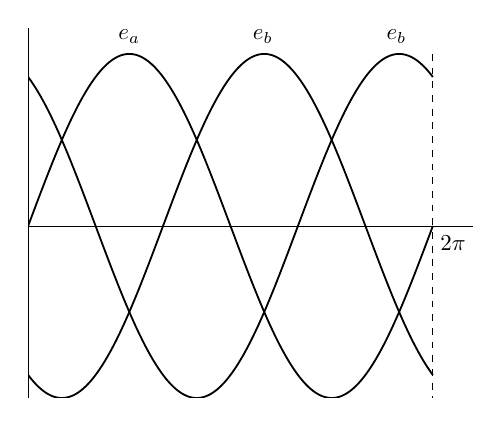
\begin{tikzpicture}[scale=0.825]
                \begin{axis}[
                domain=0:1, 
                samples=400, 
                axis lines=middle, 
                axis line style={-}, 
                xtick=\empty, 
                ytick=\empty, 
                xticklabel=\empty, 
                yticklabel=\empty,
                ymax = 1.15,
                xmax = 1.1,
                ]
                
                \addplot[black,thick] {sin(deg(2*pi*x))}; 
                \addplot[black,thick] {sin(deg(2*pi*x - 2*pi/3))}; 
                \addplot[black,thick] {sin(deg(2*pi*x + 2*pi/3))}; 
                
                \draw[dashed] (axis cs:1,1) -- (axis cs:1,-1); 
                \node at (axis cs:1.05,-0.1) {$2\pi$};
                \node at (axis cs:0.25,1.1) {$e_a$};
                \node at (axis cs:0.58,1.1) {$e_b$};
                \node at (axis cs:0.91,1.1) {$e_b$};
             \end{axis}
        \end{tikzpicture}}
        \caption{Variação no tempo das f.e.m}
    \end{figure}
    \end{minipage}%
    \begin{minipage}[b]{0.5\linewidth}
        \begin{figure}[H]
        \centering
            \scalebox{0.925}{%
            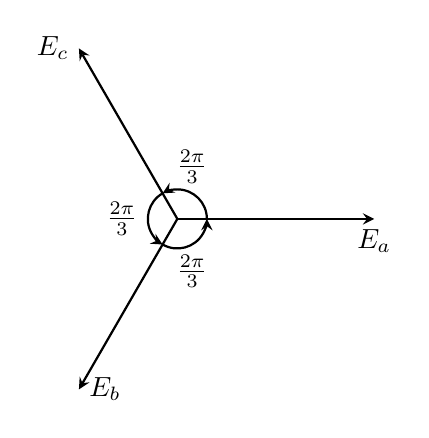
\begin{tikzpicture}[scale=1.25,>=stealth]
                 \coordinate (O) at (0,0);
        
                  \draw[->,thick] (O) -- ++(240:2cm) node[right] {$E_b$}; 
                  \draw[->,thick] (O) -- ++(360:2cm) node[below] {$E_a$}; 
                  \draw[->,thick] (O) -- ++(480:2cm) node[left] {$E_c$};
                
                  \draw[->, thick] (240:0.3cm) arc (240:360:0.3cm) node[midway, below] {$\frac{2\pi}{3}$};   
                  \draw[->, thick] (360:0.3cm) arc (360:480:0.3cm) node[midway, above] {$\frac{2\pi}{3}$};
                  \draw[->,thick] (480:0.3cm) arc (480:600:0.3cm) node[midway, left] {$\frac{2\pi}{3}$};
            \end{tikzpicture}}
        \caption{Diagrama de fasores}
        \end{figure}
    \end{minipage}
\end{centering}

%% next page
\clearpage
\begin{minipage}[c]{0.4\textwidth}
    \begin{figure}[H]
        \centering
        \begin{tikzpicture}[scale=1.5,>=stealth]
            \coordinate (O) at (0,0);
            
            \draw[->,thick] (O) -- ++(240:2cm) node[below] {$V_b$}; 
            \draw[->,thick] (O) -- ++(360:2cm) node[right] {$V_a$}; 
            \draw[->,thick] (O) -- ++(480:2cm) node[above] {$V_c$};
    
            \draw[->,thick] (O) -- ++(210:0.75cm) node[above] {$I_b$};
            \draw[->,thick] (O) -- ++(330:0.75cm) node[below] {$I_a$};
            \draw[->,thick] (O) -- ++(450:0.75cm) node[right] {$I_c$};
    
            \draw (360:0.3cm) arc (360:330:0.3cm) node[midway, right, below=, font=\small] {$\phi$};
            \draw (240:0.3cm) arc (240:210:0.3cm) node[midway, left, font=\small] {$\phi$};
            \draw (480:0.3cm) arc (480:450:0.3cm) node[midway, above, font=\small] {$\phi$};
    
            % Calculate the coordinates of the tips of V_a, V_b, and V_c
            \coordinate (tipA) at ($(O)+(360:2cm)$);
            \coordinate (tipB) at ($(O)+(240:2cm)$);
            \coordinate (tipC) at ($(O)+(480:2cm)$);
            
            % Draw vectors V_ab, V_ca, and V_bc
            \draw[->,thick,dashed] (tipB) -- (tipA) node[midway, below=0.75mm] {$V_{ab}$};
            \draw[->,thick,dashed] (tipA) -- (tipC) node[midway, above] {$V_{ca}$};
            \draw[->,thick,dashed] (tipC) -- (tipB) node[midway, left] {$V_{bc}$};
    
            % Draw the angle 
            \draw (O) ++(360:1.45cm) arc (180:210:0.55cm);
            \node at ($(O)+(351:1.3cm)$) {$\frac{\pi}{6}$};
        \end{tikzpicture}
        \caption{Fasores de tensão (simples e composta) e fasores de corrente num sistema trifásico simétrico.}
    \end{figure}
\end{minipage} \hfill
\begin{minipage}[c]{0.525\textwidth} \small
    \noindent As \textit{tensões simples} ou \textit{fase-neutro} são então: 
    $$ 
    \begin{aligned} 
        v_a &= \sqrt{2} V \sin(\omega t) \\ 
        v_b &= \sqrt{2} V \sin(\omega t - 2\pi/3) \\ 
        v_c &= \sqrt{2} V \sin(\omega t + 2\pi/3) 
    \end{aligned} 
    \qquad\rightleftarrows\qquad 
    \begin{aligned} 
        \mathbf{V}_{a} &= V e^{j0} \\ 
        \mathbf{V}_{b} &= V e^{-j2\pi/3} \\ 
        \mathbf{V}_{c} &= V e^{j2\pi/3} 
    \end{aligned} 
    $$ 
    
    Num sistema trifásico, define-se o valor das \textit{tensões fase-fase} (ou \textit{tensões entre fases} ou \textit{tensões compostas}): 
    $$ 
    \begin{aligned} 
        \mathbf{V}_{ab} &= \mathbf{V}_a - \mathbf{V}_b \\ 
        \mathbf{V}_{bc} &= \mathbf{V}_b - \mathbf{V}_c \\ 
        \mathbf{V}_{ca} &= \mathbf{V}_c - \mathbf{V}_a 
    \end{aligned} 
    \;\rightarrow\; 
    \boxed{\begin{aligned} 
        V_L &= V_{ab} = V_{bc} = V_{ca} = 2V \cos(\pi/6) \\ 
            &= \sqrt{3} V \mkern9mu\text{\small (valor eficaz das compostas)}
    \end{aligned}} 
    $$ 
    
    \noindent Uma vez que a carga é simétrica, as correntes escrevem-se: 
    $$ \begin{aligned} 
        i_a &= \sqrt{2} I \sin(\omega t - \phi) \\ 
        i_b &= \sqrt{2} I \sin(\omega t - \phi - 2\pi/3) \\ 
        i_c &= \sqrt{2} I \sin(\omega t - \phi + 2\pi/3) 
    \end{aligned} 
    \qquad\rightleftarrows\qquad 
    \begin{aligned} 
        \mathbf{I}_{a} &= I e^{-j\phi} \\ 
        \mathbf{I}_{b} &= I e^{-j(2\pi/3 + \phi)} \\ 
        \mathbf{I}_{c} &= I e^{j(2\pi/3 - \phi)} 
    \end{aligned} 
    $$
\end{minipage}

\begin{mdframed} % miminhos
    \noindent \textbf{Notas}:
    \begin{enumerate}[noitemsep,nolistsep,leftmargin=*,label=\arabic*.,font=\small\bfseries]\small
        \item ``A soma das correntes nas três fases é nula, logo não é necessário um condutor a conectar o neutro do gerador com o da carga. Os dois neutros estão ao potencial da terra, quer no gerador quer na carga.''\cite{paiva2005}
        
        \item ``Num sistema trifásico simétrico, todas as tensões simples podem ser medidas em relação a um neutro, que tem o mesmo potencial (zero) ao longo de todo o sistema.''\cite{paiva2005}
    \end{enumerate}
\end{mdframed}

%//==============================--@--==============================//%
\subsubsection{Potência Instantânea, Potência Ativa e Reativa, e Potência Complexa}

A potência transferida do gerador para a carga será a soma das potências instantâneas por fase:
$$
    p = v_a i_a + v_b i_b + v_c i_c = 3 VI \cos(\phi)
$$
Verifica-se que a \textit{potência trifásica instantânea} é constante, e igual a 3 vezes a potência ativa por fase.

Deste modo, a \textit{potência ativa trifásica} escreve-se:
$$
    P = 3 VI \cos(\phi) = \sqrt{3} V_L I \cos (\phi) \quad [\text{W}]
$$
A \textit{potência reativa trifásica} é definida como a soma algébrica das potências reativas em cada fase:
$$
    Q = 3 VI \sin(\phi) = \sqrt{3} V_L I \cos (\phi) \quad [\text{VAr}]
$$
A \textit{potências complexa e aparente para sistemas trifásicos} é dada por:
$$
\begin{aligned}
    \mathbf{S} &= 3\mathbf{V} \mathbf{I}^* = P + jQ\\
    S &= \sqrt{P^2 + Q^2} = 3VI = \sqrt{3} V_L I \quad [\text{VA}]
\end{aligned}
$$

%//==============================--@--==============================//%
\subsubsection{Carga Ligada em Triângulo}

\noindent Outra forma de ligar a carga é em \underline{triângulo}, situação em que cada impedância de carga \textbf{Z} está sujeita à tensão entre fases.

\begin{centering}
    \begin{minipage}[b]{0.4\linewidth}
        \begin{figure}[H]
        \centering
        \resizebox{0.75\textwidth}{!}{%
        \begin{circuitikz}[>=stealth]
        % Nodes
        \draw (-2,2) to[short, -*] (-2,2);
        \draw (-2,0) to[short, -*] (-2,0);
        \draw (-2,-2) to[short, -*] (-2,-2);
        
        %Lines
        \draw [](-2,0) to[short] (1,0);
        \draw (1,0) to[short, -*] (1,0);
        \draw (1,0) to[R,*-*] (2.5,2);
        \draw (1,0) to[R,*-*] (2.5,-2);
        \draw (2.5,2) to[R,*-*] (2.5,-2);
        \draw (-2,2) to[short, -*] (2.5,2);
        \draw (-2,-2) to[short, -*] (2.5,-2);
        
        \node at (3,0) {$Z_\Delta$};
        \node at (1.1,1) {$Z_\Delta$};
        \node at (1.1,-1) {$Z_\Delta$};
        
        \node[coordinate,label=left:$a$] at (-2,2) {};
        \node[coordinate,label=left:$b$] at (-2,0) {};
        \node[coordinate,label=left:$c$] at (-2,-2) {};
        
        % Arrows
        \draw[->,thick](-2, 1.8) to[short] (-2,0.2);
        \draw[->,thick](-2, -0.2) to[short] (-2,-1.8);
        \draw[->,thick](-2.5, -1.8) to[short] (-2.5,1.8);
        
        \node at (-2.9,0) {$V_{ca}$};
        \node at (-1.7,1) {$V_{ab}$};
        \node at (-1.7,-1) {$V_{bc}$};
        
        \draw[->,thick](0, 2) to[short] (0.1,2) node[above] {$I_a$};
        \draw[->,thick](0, 0) to[short] (0.1,0) node[above] {$I_b$};
        \draw[->,thick](0, -2) to[short] (0.1,-2) node[above] {$I_c$};
        
        \draw[->,thick](2.5, -1.5) to[short] (2.5,-1.3) node[right=0.1] {$I_{ca}$};
        
        
        \end{circuitikz}
        }%
        \caption{Carga ligada em triângulo.}
        \end{figure}
\end{minipage}%
    \begin{minipage}[b]{0.6\linewidth}
        \begin{mdframed}
            \noindent As correntes $\bar{I}_{ab}$, $\bar{I}_{bc}$ e $\bar{I}_{ca}$ são:
            \vspace{0.5em}
            $$
                \bar{I}_{ab} = \dfrac{\overline{V}_{ab}}{\overline{Z}_\Delta}\quad
                \bar{I}_{bc} = \dfrac{\overline{V}_{bc}}{\overline{Z}_\Delta}\quad
                \bar{I}_{ac} = \dfrac{\overline{V}_{ac}}{\overline{Z}_\Delta}
            $$
            \vspace{0.5em}
            \noindent A corrente na linha $I_a$ é, por conseguinte:
            $$
                \boxed{\bar{I}_a = \dfrac{\overline{V}_{ab} - \overline{V}_{ca}}{\overline{Z}_\Delta} = \dfrac{3\overline{V}_a}{\overline{Z}_\Delta}}
            $$
            \noindent A amplitude da corrente é \textbf{3 vezes maior} que na ligação da carga em estrela.
        \end{mdframed}
    \end{minipage}
\end{centering}

\noindent A \underline{potência absorvida} pela carga ligada em triângulo é \textbf{3 vezes maior} que a ligada em estrela, para o mesmo valor de impedância de carga.

%//==============================--@--==============================//%
\paragraph{Conversão entre Ligação em Estrela e Ligação em Triângulo (wye $\rightleftarrows$ delta)}

\begin{table}[ht]
    \centering
    \caption{Transformações Y-$\Delta$ e $\Delta$-Y}

    \setlength{\tabcolsep}{1cm}
    
    \begin{tabular}{cc}
        \begin{circuitikz}
            \ctikzset{resistors/scale=0.75}
            
            % Define interest points
            \coordinate (A) at (0,0);
            \coordinate (B) at (4,0);
            \coordinate (C) at (2,{-2*sqrt(3)});
            \coordinate (G) at (2,{-(2/3)*sqrt(3)});
    
            % Draw the skeleton
            \draw[dashed] (A) -- (G) -- (B);
            \draw[dashed] (G) -- (C);
    
            \node[circ] at (A) {};
            \node[circ] at (B) {};
            \node[circ] at (C) {};
            \node[circ] at (G) {};

            \node[left] at (A) {$a$};
            \node[right] at (B) {$b$};
            \node[below] at (C) {$c$};
    
            % Draw the impedances
            \draw (A) to[R, a=$Z_{ab}$] (B) to[R, a=$Z_{bc}$] (C) to[R, a=$Z_{ca}$] (A);
        \end{circuitikz}
        &
        \begin{circuitikz}
            \ctikzset{resistors/scale=0.75}
            
            % Define interest points
            \coordinate (A) at (0,0);
            \coordinate (B) at (4,0);
            \coordinate (C) at (2,{-2*sqrt(3)});
            \coordinate (G) at (2,{-(2/3)*sqrt(3)});
    
            % Draw the skeleton
            \draw[dashed] (A) -- (B) -- (C) -- (A);
            \node[circ] at (A) {};
            \node[circ] at (B) {};
            \node[circ] at (C) {};
            \node[circ] at (G) {};

            \node[left] at (A) {$a$};
            \node[right] at (B) {$b$};
            \node[below] at (C) {$c$};
            
            % Draw the impedances
            \draw (A) to[R, l=$Z_{a}$] (G) to[R, l=$Z_{b}$] (B);
            \draw (C) to[R, l=$Z_{c}$] (G);
        \end{circuitikz} \\
        $\begin{aligned}
            \boxed{\textbf{Y} \to \mathbf{\Delta}}\\
            Z_{ab} &= \frac{Z_aZ_b+Z_bZ_c+Z_cZ_a}{Z_c} \\
            Z_{bc} &= \frac{Z_aZ_b+Z_bZ_c+Z_cZ_a}{Z_a} \\
            Z_{ca} &= \frac{Z_aZ_b+Z_bZ_c+Z_cZ_a}{Z_b}
        \end{aligned}$
        & 
        $\begin{aligned}
            \boxed{\mathbf{\Delta} \to \textbf{Y}}\\
            Z_a &= \frac{Z_{ab}Z_{ca}}{Z_{ab}+Z_{bc}+Z_{ca}} \\
            Z_b &= \frac{Z_{bc}Z_{ab}}{Z_{ab}+Z_{bc}+Z_{ca}} \\
            Z_c &= \frac{Z_{ca}Z_{cb}}{Z_{ab}+Z_{bc}+Z_{ca}}
        \end{aligned}$ 
    \end{tabular}
\end{table}

%//==============================--@--==============================//%
\vspace*{-1em}%
\subsection{Valores por Unidade}

O uso de \textit{valores por unidade} (p.u.) consiste na quantificação das grandezas elétricas como frações de valores de base, designados por valores nominais ou de plena carga. O valor p.u. de uma grandeza obtém-se por
$$
    \text{valor p.u.} = \frac{\text{valor da grandeza}}{\text{valor da base}}
$$
\textbf{Nota}: O valor da grandeza pode ser um fasor/número complexo ou um valor instantâneo em unidades SI, enquanto o valor de base é um número real adequado. O valor de base pode ser \underline{postulado} ou \underline{derivado}.

%//==============================--@--==============================//%
\subsubsection{Sistemas Monofásicos}

\begin{mdframed}
    \noindent Num sistema monofásico, postula-se: 
    \begin{center}
        a \textit{base de tensão} $[$kV$]$, $V_b$ e a \textit{base de potência} $[$MVA$]$, $S_b$
    \end{center}
    \noindent Os valores de base derivados são:
    \begin{itemize}[noitemsep,label=-,font=\bfseries]
        \item \textit{base de corrente} $[$kA$]$, $$ I_b = S_b/V_b $$
        \item \textit{base de impedância} $[\Omega]$, $$ Z_b = V_b/I_b = V^2_b/S_b $$
        \item \textit{base de admitância} $[$S$]$, $$ Y_b = I_b/V_b = S_b/V^2_b$$
    \end{itemize}
\end{mdframed}

%//==============================--@--==============================//%
\subsubsection{Sistemas Trifásicos}

\begin{mdframed}
Analogamente, postula-se para base a tensão \underline{entre fases}, $V_b$, e a potência aparente \underline{trifásica}, $S_b$.

\vspace{1em}
\noindent Temos a relação $S_b = \sqrt{3} V_b I_b$, de onde se derivam as restantes:
\begin{itemize}[noitemsep,label=-,font=\bfseries]
        \item \textit{base de corrente} $[$kA$]$, $$ I_b = S_b/\sqrt{3}V_b $$
        \item \textit{base de impedância} $[\Omega]$, $$ Z_b = V_b/\sqrt{3}I_b = V^2_b/S_b $$
        \item \textit{base de admitância} $[$S$]$, $$ Y_b = \sqrt{3}I_b/V_b = S_b/V^2_b$$
    \end{itemize}
\end{mdframed}

%//==============================--@--==============================//%
\subsection{Transmissão de Energia}
\subsubsection{Corrente Alternada}
Considerando uma linha de transmissão de energia modelada por um elemento indutivo com reatância $X_L$, pretende-se estabelecer a relação entre as potências ativa e reativa que transitam na linha e as tensões nos nós entre as quais ela está ligada.

\vspace{-0.5em}
\begin{centering}
    \begin{minipage}[b]{0.5\linewidth}
        \begin{figure}[H]
        \centering
        \resizebox{0.8\textwidth}{!}{%
        \begin{circuitikz}[>=stealth]
        
        % Inductor
        \draw (0,0) to[cute inductor] (3,0);
        \node at (1.5,0.4) {$j X_L$};
        
        % Nodes
        \draw (0, 0) to[short, -*] (0,0);
        \draw (3,0) to[short, -*] (3,0);
        \draw (0,-2) to[short, -*] (0,-2);
        \draw (3,-2) to[short, -*] (3,-2);
        
        % Wire
        \draw (0, -2) to[short, -*] (3,-2);
        
        % Arrows
        \draw[->,thick](0, -0.2) to[short] (0,-1.8);
        \node at (-0.3,-1) {$V_1$};
        
        \draw[->,thick](3, -0.2) to[short] (3,-1.8);
        \node at (3.3,-1) {$V_2$};
        
        \draw[->,thick](0.5, 0) to[short] (0.55,0) node[above] {$I$};
        
        \end{circuitikz}
        }%
        \caption{Transmissão de energia --- elemento indutivo.}
        \end{figure}
\end{minipage}%
    \begin{minipage}[b]{0.5\linewidth}
        \begin{mdframed}
            A corrente que percorre a linha, definida como positiva no sentido $1 \rightarrow 2$:
            $$
                I = \dfrac{V_1 - V_2}{j X_L}
            $$
            A potência complexa $\mathbf{S}_{12}$:
            $$
            \begin{aligned}
                &\mathbf{S}_{12} = \mathbf{V_1} \mathbf{I^*} = \mathbf{V_1}\dfrac{ \mathbf{V}_1^* -  \mathbf{V}_2^*}{-j X_L} =\\ &\dfrac{ V_1^2 - \mathbf{V}_1\mathbf{V}_2^*}{-j X_L}\quad\text{em que}\quad
                \left\{\begin{aligned}
                    \mathbf{V}_1 &= V_1 e^{j\theta_1} \\
                    \mathbf{V}_2 &= V_2 e^{j\theta_2}
                \end{aligned}\right.
            \end{aligned}
            $$
        \end{mdframed}
    \end{minipage}
\end{centering}

\noindent Seja $\theta = \theta_1 - \theta_2$ o ângulo de desfasagem entre as tensões no nó 1 e no nó 2:
$$
\mathbf{S_{12}} = j\dfrac{ V_1^2 -  V_1 V_2 e^{j\theta}}{X_L} = \underbrace{\dfrac{V_1 V_2 \sin(\theta)}{X_L}}_{P_{12}} + \underbrace{j \dfrac{V_1^2 - V_1 V_2 \cos(\theta)}{X_L}}_{Q_{12}}
$$
De forma análoga se deduzem as potência ativa e reativa na receção, positivas no sentido $2 \rightarrow 1$:
$$
P_{21} = - \dfrac{V_1 V_2 \sin(\theta)}{X_L}\qquad 
Q_{21} = \dfrac{V_2^2 - V_1 V_2 \cos(\theta)}{X_L}
$$
Somando as duas equações vem que:
$$
\begin{aligned}
    &P_L = P_{12} + P_{21} = 0\\
    &Q_L = Q_{12} + Q_{21} = \dfrac{V_1^2 + V_2^2 - 2 V_1 V_2 \cos(\theta)}{X_L}
\end{aligned}
$$
em que $P_L$ e $Q_L$ representam as perdas de potência ativa e reativa na linha. Uma vez que desprezamos a resistência, as perdas de potência ativa são nulas. As perdas de potência reativa não correspondem a perdas energéticas, no entanto, \underline{o balanço da potência reativa deve de ser fechado}\footnotemark[1] como a potência ativa.

\footnotetext[1]{%
    Caso contrário, o desequilíbrio provocará flutuações nas tensões em diferentes partes do sistema, que levam a ineficiências energéticas. 
}

\begin{mdframed}
   \noindent \textbf{Notas}:
    \begin{enumerate}[nolistsep,noitemsep,leftmargin=*,label=\arabic*.,font=\small\bfseries]\small
        \item O sentido do trânsito de potência ativa é determinado pelo ângulo de desfasagem $\theta$ entre as tensõe de cada nó.
        
        \item As amplitudes das tensões $V_1$ e $V_2$ influenciam o sentido de trânsito da potência reativa. Caso as tensões sejam de igual amplitude nos dois extremos $V_1 = V_2 = V_n$ (tensão nominal), então:
        $$
            Q_{\textit{med}} = \dfrac{Q_{12} - Q_{21}}{2} = 0
        $$
        O mesmo não acontece com o balanço de potência reativa $Q_L = Q_{12} + Q_{21}$, uma vez que os valores nos extremos não se anulam, i.e., $Q_{12} = Q_{21} = V^2_n (1-\cos(\theta))/X_L$. O que leva a 
        $$
            Q_L = \frac{2V^2_n (1-\cos(\theta))}{X_L}
        $$
    \end{enumerate} 
\end{mdframed}

%//==============================--@--==============================//%
\subsection{Caracterização das Cargas}

As cargas típicas têm \underline{caráter indutivo}, e agrupam-se em quatro tipos: (i) motores, (ii) iluminação, (iii) aquecimento e refrigeração e (iv) aparelhos eletrónicos. Normalmente são caracterizadas pela potência ativa $P_C$ e pela potência reativa $Q_C$ ou fator de potência $\cos(\phi)$ (alternativamente poderá utilizar-se $\tan(\phi)$):
$$
    \cos(\phi) = \frac{P_C}{\sqrt{P^2_C + Q^2_C}} \quad \land \quad \tan(\phi) = \frac{P_C}{Q_C}
$$

%//==============================--@--==============================//%